\documentclass[justified]{tufte-handout}

% ams
\usepackage{amssymb,amsmath}

\usepackage{ifxetex,ifluatex}
\usepackage{fixltx2e} % provides \textsubscript
\ifnum 0\ifxetex 1\fi\ifluatex 1\fi=0 % if pdftex
  \usepackage[T1]{fontenc}
  \usepackage[utf8]{inputenc}
\else % if luatex or xelatex
  \makeatletter
  \@ifpackageloaded{fontspec}{}{\usepackage{fontspec}}
  \makeatother
  \defaultfontfeatures{Ligatures=TeX,Scale=MatchLowercase}
  \makeatletter
  \@ifpackageloaded{soul}{
     \renewcommand\allcapsspacing[1]{{\addfontfeature{LetterSpace=15}#1}}
     \renewcommand\smallcapsspacing[1]{{\addfontfeature{LetterSpace=10}#1}}
   }{}
  \makeatother

\fi

\usepackage{graphicx}
\setkeys{Gin}{width=\linewidth,totalheight=\textheight,keepaspectratio}
\usepackage{booktabs}
\usepackage{url}
\usepackage{hyperref}
\usepackage{units}


\setcounter{secnumdepth}{2}

\usepackage{multicol}
\usepackage[normalem]{ulem}
\usepackage{morefloats}

% tightlist macro required by pandoc >= 1.14
\providecommand{\tightlist}{%
  \setlength{\itemsep}{0pt}\setlength{\parskip}{0pt}}

% title / author / date
\title{Big Data Computing cluster - admin guide}
\author{Matteo Ceccarello}
\date{}


\begin{document}

\maketitle

{
\setcounter{tocdepth}{3}
\tableofcontents
}

\vspace{1em}

This document describes how to manage and set up the cluster for the Big
Data course on CloudVeneto.

\section{Structure of the cluster}\label{structure-of-the-cluster}

The cluster consists of 10 virtual machines: one machine called
\texttt{frontend} and nine machines called \texttt{minion-1} to
\texttt{minion-9}. The \texttt{minion-*} machines are responsible for
running the workers that execute the code of the students. The
\texttt{frontend} machine has a coordinating role: students submit their
jobs to \texttt{frontend}, which then schedules them for executions
using the available resources. The \texttt{frontend} machine is the only
one the students have access to.

The machines are connected with the network \texttt{10.67.13.*}. Since
the students need to have access from the outside, we the CloudVeneto
admins configured for us a \emph{public IP} (\texttt{147.162.226.106})
which allows to log to \texttt{frontend} without going through the
CloudVeneto gate. This IP is accessible from the Unipd networks (so the
internal DEI network, the internal network of the Math department, and
similar) but not from the outer Internet. Therefore if the students want
to log in from home, they first need to \texttt{ssh} to
\texttt{login.dei.unipd.it} (or the equivalent for their department).

\section{Preliminary steps}\label{preliminary-steps}

Before starting, make sure that you have the private key to access the
cluster in your \texttt{\textasciitilde{}/.ssh} directory. This key,
named \texttt{cloudveneto-machines.pem}, was generated by CloudVeneto
when the Big Data Computing project was created, and is needed to access
the machines when they are created, before we can configure other means
of logging in. It's not clear to me how to replace it, so we should pay
attention not to lose it.

The configuration of the cluster is done with Ansible, which can be
installed following
\href{https://docs.ansible.com/ansible/latest/installation_guide/intro_installation.html}{these
instructions}. To use Ansible, as well as some other scripts, you will
need a working Python 3 installation. To verify this, make sure that the
following command succeeds:

\begin{verbatim}
python3 -V
\end{verbatim}

As the last preliminary step, clone the git repository available at
https://github.com/Cecca/big-data-course on your machine\footnote{This
  repository is private on GitHub, and every user needs to be granted
  access.}:

\begin{verbatim}
git clone git@github.com:Cecca/big-data-course.git
\end{verbatim}

This guide assumes a UNIX-like machine (i.e.~Linux or MacOS).

\section{Setting up the cluster}\label{setting-up-the-cluster}

This section will walk through the setup of the cluster.

\subsection{Creating the machines}\label{creating-the-machines}

The machines are created using the
\href{https://cloudveneto.ict.unipd.it/dashboard}{dashboard}. Go to the
\emph{instances} tab, and click the \emph{Launch instance} button. A
dialog with several options.

All machines should be created using the following setup (settings not
mentioned here are to be left at the defaul values):

\begin{itemize}
\tightlist
\item
  Flavor: \texttt{cloudveneto.xlarge}
\item
  Instance boot source: \texttt{boot\ from\ image}
\item
  Image name: \texttt{ubuntu-16.04-java8-spark-2.2.0}\ldots{} \footnote{To
    create the image file, see Appendix \ref{sec:creating-images}. For
    our purposes, the already existing image should be fine.}
\end{itemize}

For the \texttt{frontend} machine, the \emph{Instance name} field should
be set to \texttt{frontend}, for the others \texttt{minion-x} should be
used, with \texttt{x} replaced by the appropriate number\footnote{The
  minions can also be created all in one go, by changing the
  \emph{Number of instances} field in the dialog.}.

The dialog to launch the minion machines is shown in the following
figure. Note that here we are creating all 9 minion machines in one go:
the name we set in the dialog is \texttt{minion}, then CloudVeneto will
take care of appending \texttt{-i} to the name, with \(i \in [1,9]\).
For the \texttt{frontend} machine the settings are the same except for
the name and the number of instances.

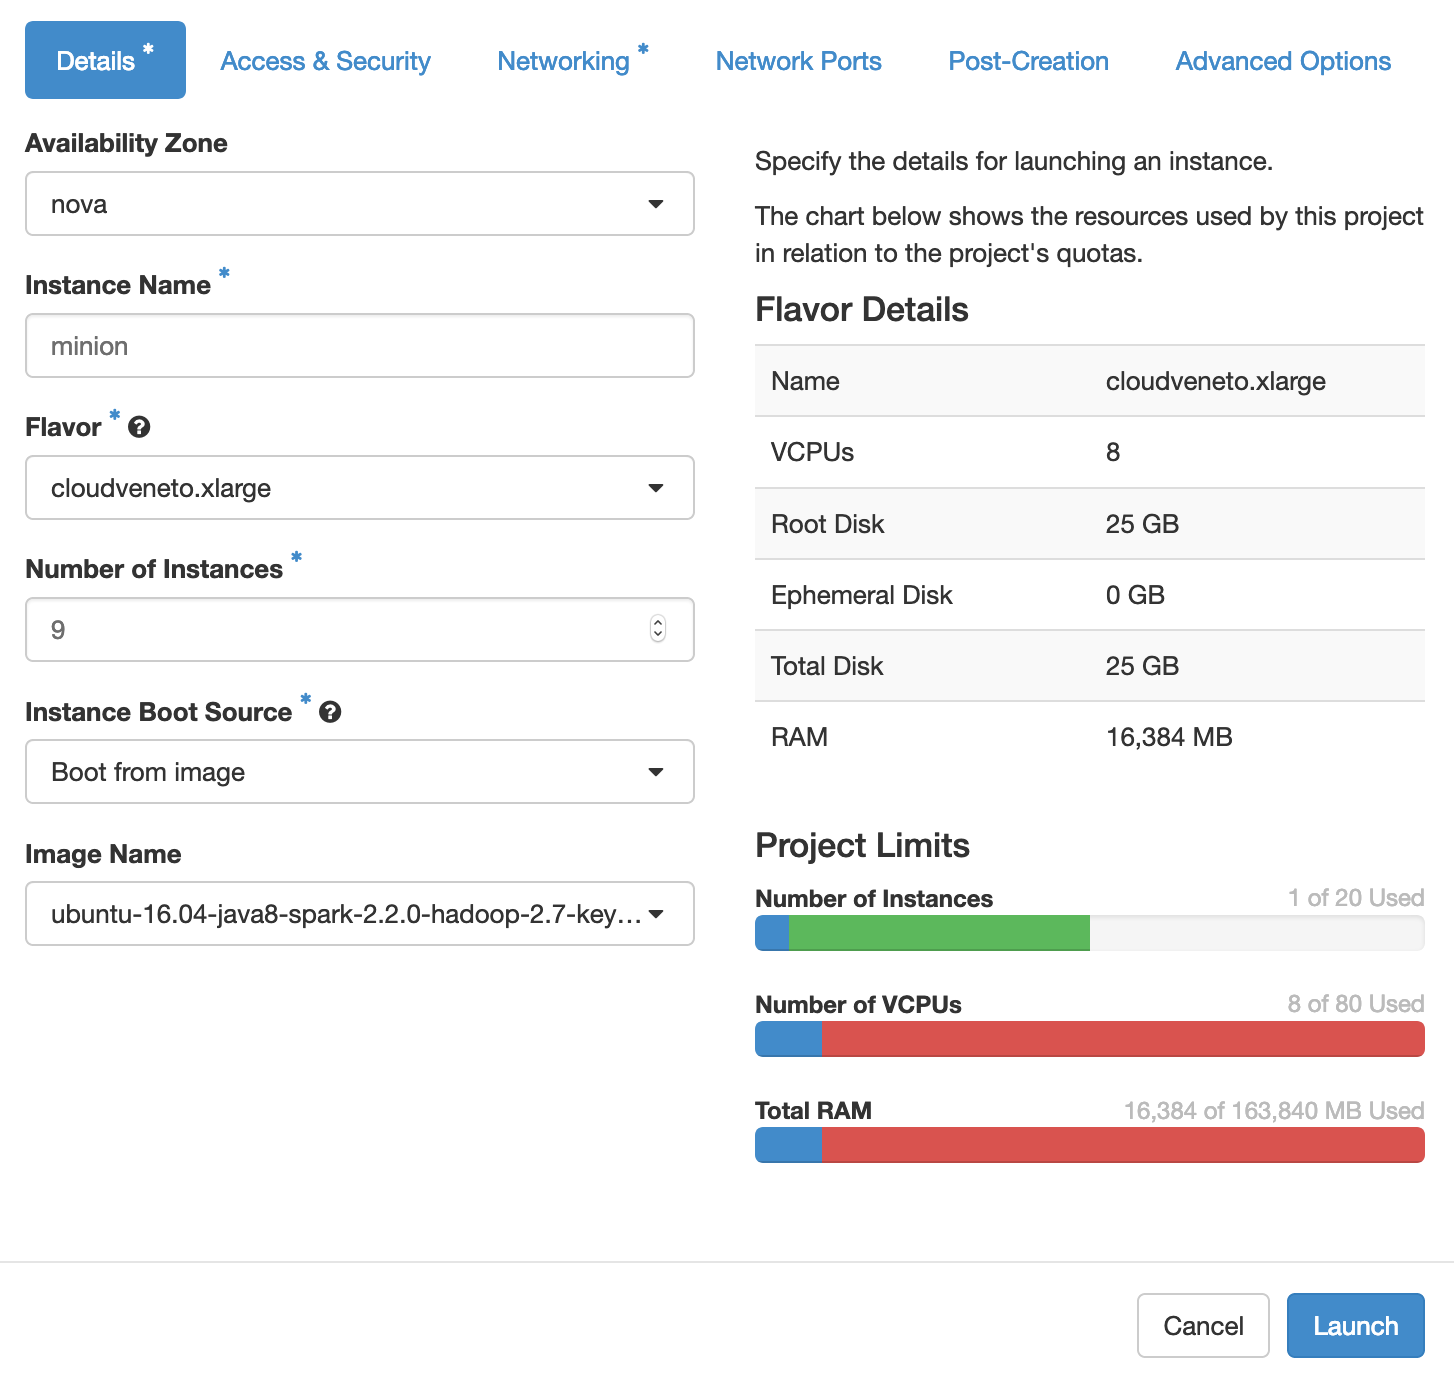
\includegraphics{screens/launch-minions.png}\\
After waiting a while, the machines should be set up, and you should be
presented with the following screen. At this point the machines are
running, they have Spark, Yarn, and HDFS installed, but they still don't
know about each other. Configuring networking, among other things, will
be the topic of the next section. Take note of the IP addresses of the
machines, as reported on the dashboard. The dashboard should present you
with a situation similar to this: the red rectangle highlight the IP
addresses you need to take note of.

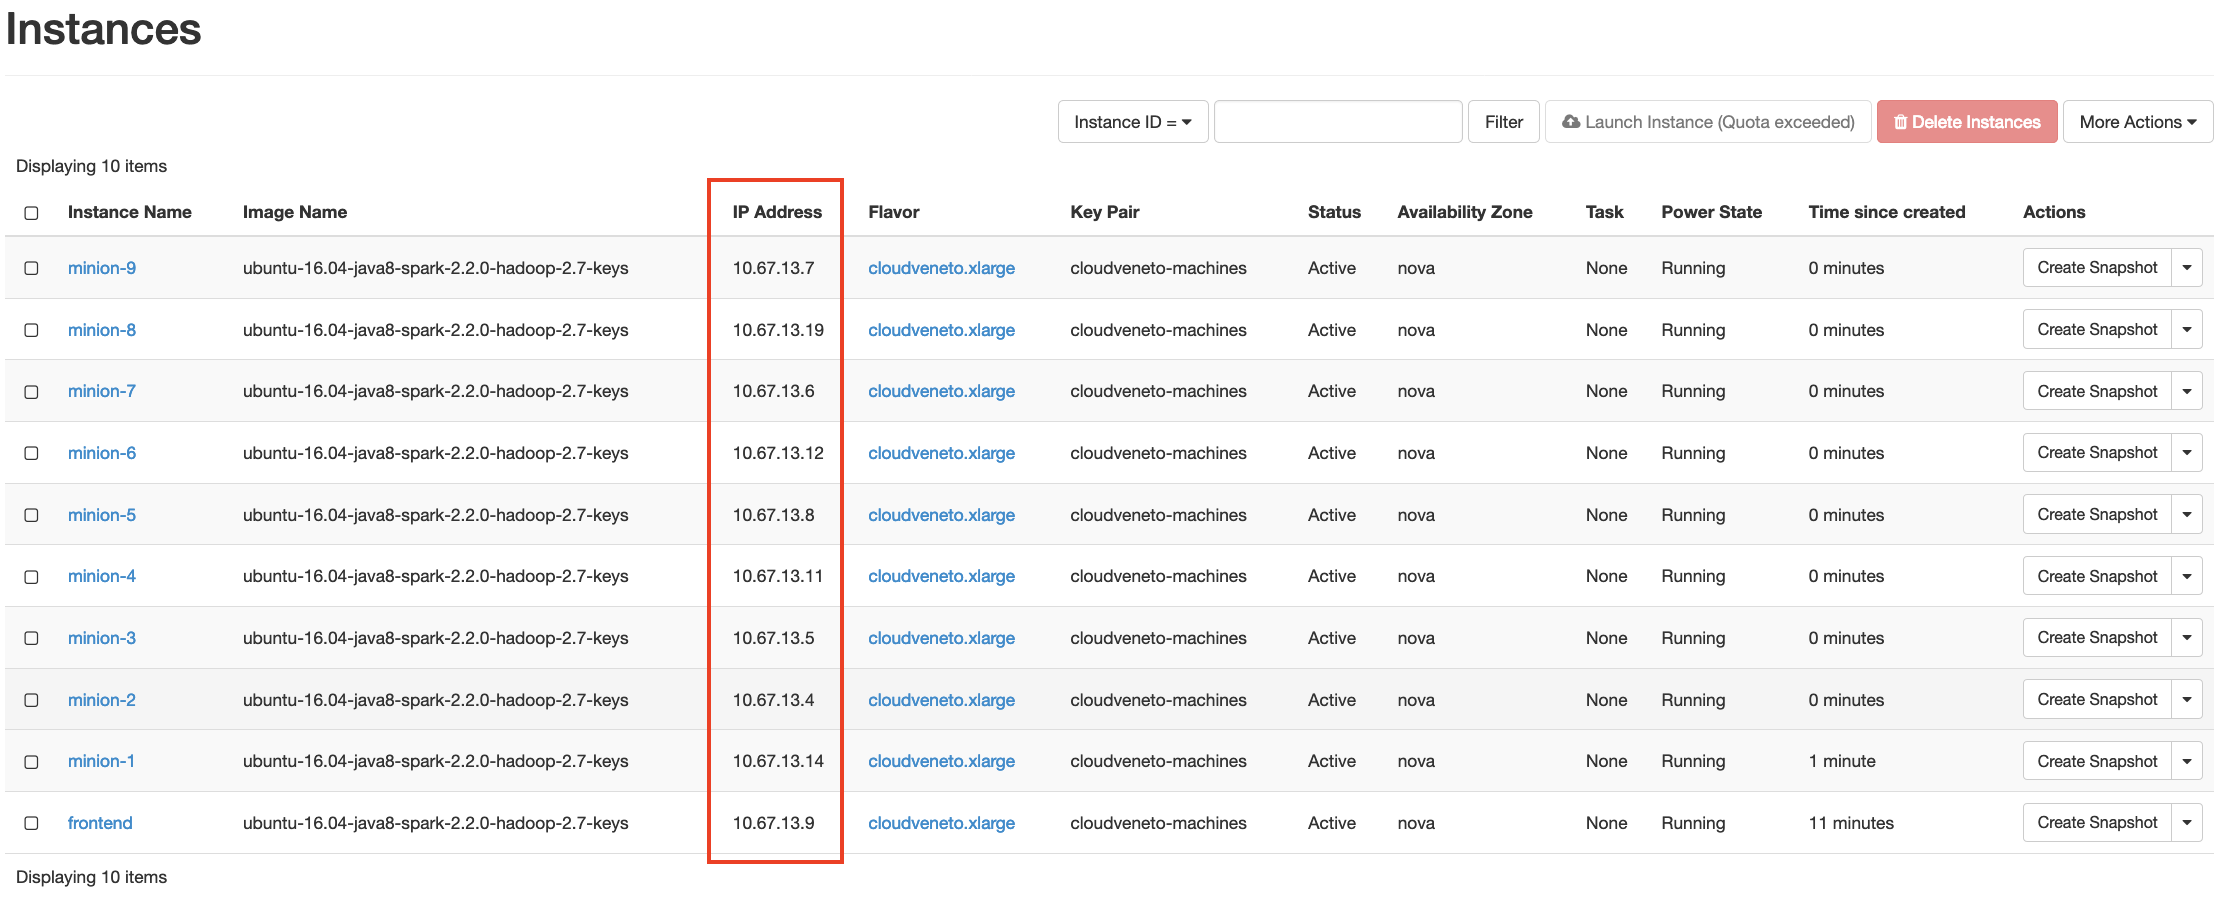
\includegraphics{screens/launched-machines.png}\\

Before proceeding, we need to configure networking on the CloudVeneto
side. Go to the \emph{network} tab of the dashboard and select
\emph{Security groups}\footnote{Security groups act as some sort of
  \emph{firewall} for incoming connections. The defaults should be
  tweaked in order to make basic features work, such as SSH login
  without going through CloudVeneto's gate.}. There should be just one
security group, the default one.

We will need to set several rules. For all of them, leave the defaults
in the dialog except for the \texttt{port} field. The defaults are:

\begin{itemize}
\tightlist
\item
  Rule: custom TCP Rule
\item
  direction: Ingress
\item
  Open Port: Port
\item
  Remote: CIDR
\item
  CIDR: 0.0.0.0/0
\end{itemize}

Then we need to create a rule for each of these ports (if they are not
already present):

\begin{itemize}
\tightlist
\item
  2222 (additional ssh port)
\item
  8088 (YARN web interface)
\item
  18080 (Spark History server)
\item
  50070 (HDFS web interface)
\end{itemize}

Now we have that the \texttt{frontend} machine running, and the security
groups configured, we can associate the public IP to the
\texttt{frontend} machine\footnote{Normally machines on CloudVeneto are
  accessible just from CloudVeneto's own gate. This is very inconvenient
  for our setup, since it requries to have an account on CloudVeneto for
  each user. Using a Public IP (also called \emph{floating IP}) allows
  to bypass CloudVeneto's gate.}. Click on the \emph{Floating IPs} tab.
There should be a single IP address shown. Click on the button at the
end of the line, and associate it to the \texttt{frontend} machine.

Now we are ready to test the connectivity of the machines. First we
should log into CloudVeneto's gate and then, from there, to the
frontend.

\begin{verbatim}
ssh -i ~/.ssh/cloudveneto-machines.pem mceccare@gate.cloudveneto.it
ssh -i ~/.ssh/cloudveneto-machines.pem ubuntu@10.67.13.9
\end{verbatim}

Replace \texttt{mceccare} with your username. Do not replace
\texttt{ubuntu}, instead. That's the default user name available on the
machines, we are going to use it for the administrative steps. Note that
the IP address of the frontend in the second step might be different.
You can also verify access to the other machines at this point, if you
want.

Before proceding, we have to setup the frontend to accept \texttt{ssh}
connections coming on the public IP on the port 2222. Log in to
\texttt{frontend} and edit the file \texttt{/etc/ssh/sshd\_config}.

\begin{verbatim}
sudo vim /etc/ssh/sshd_config
\end{verbatim}

One of the first lines is \texttt{Port\ 22}. Just below that line, add
another one stating: \texttt{Port\ 2222}. This will make the
\texttt{ssh} daemon listen on both ports 22 and 2222. Save and close the
file, and restart the \texttt{ssh} daemon:

\begin{verbatim}
sudo service sshd restart
\end{verbatim}

\vspace{2em}

Finally, we need to setup the external disks of each host. Go to the
\emph{Volumes} tab of the dashboard and, using the \emph{Create volume}
button create one disk of type \texttt{equallogic-unipd}, named
\texttt{HDFS} of size \texttt{550Gb}. Then, create other 9 disks named
\texttt{spark-scratch-1},\ldots{}, \texttt{spark-scratch-9} of size
\texttt{50Gb} each. Once all the volumes have been created, we must
attache them to the machines. To attach a volume to a machine, you have
to select the drop down menu, as shown in
Figure~\ref{fig:manage-attachments}. Attach volume HDFS to the frontend,
and all other volumes to a minion each.

\begin{marginfigure}[0em]
\caption{Dropdown menu for managing volumes.\label{fig:manage-attachments}}
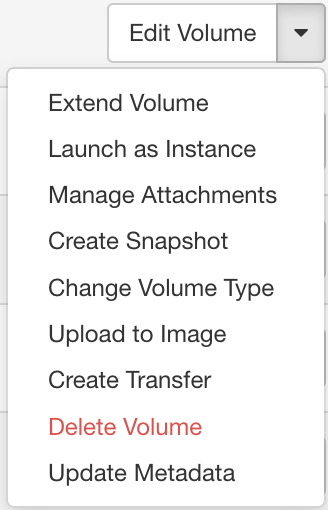
\includegraphics{screens/manage-attachments.png}
\end{marginfigure}

\subsection{~Configuring the machines with
Ansible}\label{configuring-the-machines-with-ansible}

Maintaining the configuration of all the machines of the cluster can be
challenging. To help with this task, we are using
\href{https://docs.ansible.com/}{Ansible}, which is a tool to automate
the configuration of clusters of servers. In a nutshell, this system
specifies the configuration in a series of files that describe the
\emph{desired} state of the system. The tool will then go through each
such file, checking that each host cplies with the specification. If
not, it will update the host's state.

In our case, the configuration files are in the \texttt{ansible}
directory of the repository. To deploy the configuration on the cluster
some preliminary steps are needed.

Except otherwise specified, the commands listed in this section are run
from the base directory of the repository cloned in the preliminary
steps.

\subsection{Setting up users for
groups}\label{setting-up-users-for-groups}

Users are managed using Ansible too. The configuration of Ansible is
automated with a script that can be run as follows.\footnote{To use the
  script you need the \texttt{passlib} python library installed on your
  machine. You can install it running the
  \texttt{pip3\ install\ -\/-user\ passlib} command.} If you want to
create 30 usernames, ranging from \texttt{group01} to \texttt{group30},
the only command needed is\footnote{\sloppy Note that the file
  \texttt{ansible/usernames.yml} already exists: you should
  \emph{append} the output of the above command to it, rather than
  overwriting.}

\begin{verbatim}
python3 ansible/create_groupsdata.py 30 >> ansible/usernames.yml
\end{verbatim}

Each user by default will have a password following the following
pattern: \texttt{groupXXpwd}, where \texttt{XX} is the group's name.
Users should then change their password with the \texttt{passwd}
command.

\subsection{Tell the system about the IP addresses of the
machines}\label{tell-the-system-about-the-ip-addresses-of-the-machines}

Edit the file \texttt{frontend-public.txt}, inserting as the sole
content the \emph{public IP} address of the frontend. Then, edit the
file \texttt{hosts.txt}, one line for each machine in the form
\texttt{hostname\ IP}, like in the following:

\begin{verbatim}
frontend 10.67.13.9
minion-1 10.67.13.14
minion-2 10.67.13.4
minion-3 10.67.13.5
minion-4 10.67.13.11
minion-5 10.67.13.8
minion-6 10.67.13.12
minion-7 10.67.13.6
minion-8 10.67.13.19
minion-9 10.67.13.7
\end{verbatim}

Note that for the frontend we want to use the IP of the private network
of the cluster (which is the one sharing the prefix with the minions),
not the public one.

The public IP of the frontend should instead be added to the
\texttt{frontend-public.txt} file, which should look like the following:

\begin{verbatim}
147.162.226.106
\end{verbatim}

At this point, run the script \texttt{gen-ssh-config.py} as follows

\begin{verbatim}
python3 gen-ssh-config.py >> ~/.ssh/config
\end{verbatim}

\noindent
This will append to your ssh configuration file the information needed
to access all the hosts directly using the frontend as a proxy. That is,
you can now run successfully

\begin{verbatim}
ssh minion-2
\end{verbatim}

\noindent and similar commands. Log in to each and every of the
machines, accepting their certificates. This is needed so not to have to
accept certificates later on, when other operations are running.

\vspace{1em} Now we need to populate the list of hosts to be used by
Ansible. Simply execute the following command:

\begin{verbatim}
bash gen-hosts.sh > hosts
\end{verbatim}

To check that everything is correctly configured, execute the following
command

\begin{verbatim}
ansible -i hosts all -m ping
\end{verbatim}

\noindent
all the machines should reply \texttt{pong}, with green messages.

Now we should be all set to configure the cluster. Just run

\begin{verbatim}
ansible-playbook -i hosts -b ansible/site.yml
\end{verbatim}

and wait (quite a long time) for the configuration to finish.

\vspace{2em}

To verify that Spark works, run the following command on
\texttt{frontend}, using a user other than \texttt{ubuntu}:

\begin{verbatim}
/opt/spark/bin/run-example SparkPi 10
\end{verbatim}

\section{Turning machines on and off}\label{turning-machines-on-and-off}

To turn on and off machines, go to the dashboard, select the
\emph{instances} tab, and use the dropdown menu associated to each
machine to turn them on and off, and also for rebooting.

When a machine turns on, all the associated services should start as
well, including Spark, Yarn, and HDFS. If they don't, consult the next
section on general administration.

\section{~General administration}\label{general-administration}

This section contains instructions for some common administrative stuff.
For convenience, add the following line to your
\texttt{\textasciitilde{}/.bashrc} file on the \texttt{frontend} node,
so to have Yarn, HDFS and Spark commands available

\begin{verbatim}
export PATH=$PATH:/opt/hadoop/bin:/opt/spark/bin
\end{verbatim}

\subsection{Starting Spark services}\label{starting-spark-services}

Spark-related services should start along with the machines. If they
don't, run the command

\begin{verbatim}
ansible-playbook -i hosts -b ansible/spark.yml
\end{verbatim}

\noindent
which will reconfigure the machines that are possibly misconfigured, and
will start the needed services as well.

\subsection{~Dealing with the distributed
filesystem}\label{dealing-with-the-distributed-filesystem}

Spark works best when input files are on the HDFS distributed
filesystem. In our setting we have HDFS running in a non distributed
mode, for simplicity as well as for lack of resources. A single node,
the \texttt{frontend} acts as both the \emph{namenode}\footnote{Responsible
  of maintaining metadata for files.} and the single
\emph{datanode}\footnote{Responsible of maintaining the data itself, in
  the form of blocks.}. HDFS is configured automatically along with all
the other services with Ansible.

Interaction with HDFS happens using the \texttt{/opt/hadoop/bin/hdfs}
command. The following is a brief synopsis of the most useful commands
available:

\begin{itemize}
\tightlist
\item
  \texttt{hdfs\ dfs\ -ls}: lists files under the given path (the user's
  HDFS home if none is given).
\item
  \texttt{hdfs\ dfs\ -mkdir}: makes a new directory.
\item
  \texttt{hdfs\ dfs\ -put\ SOURCE\ DEST}: copies the file
  \texttt{SOURCE} from the local filesystem to \texttt{DEST} on HDFS.
\item
  \texttt{hdfs\ dfs\ -get\ SOURCE}: copies the file (or directory) from
  HDFS to the current directory on the local filesystem.
\item
  \texttt{hdfs\ dfs\ -chown}: changes owner of a file or directory
\item
  \texttt{hdfs\ dfs\ -chmod}: changes mode of a file or directory
\end{itemize}

On the cluster, we maintain the following structure for the HDFS
filesystem

\begin{verbatim}
/
|-- data             # read-only inputs
|-- tmp              # temporary data
|-- shared           # system-generated information (Spark history)
|-- libs             # common libraries to all jobs, to reduce the startup time
|-- users            # for user generated data
    |-- group01
    |-- group02
    |-- group03
    |-- ....
    |-- groupXX
\end{verbatim}

There are two directories that are of particular interest:
\texttt{/data}, to which students have read only access, and
\texttt{/users/group*}, where students can write their own data if they
need.

An operation that is not necessary is the storage of the common
libraries in the \texttt{/shared} directory on HDFS. This will improve
the launch time for jobs, which otherwise have to copy the libraries on
the distributed file system at every run. To copy these files, execute
the following command on the fronted node:

\begin{verbatim}
hdfs dfs -ls /libs/spark-* || hdfs dfs -put /opt/spark/jars/* /libs
\end{verbatim}

This command first checks that the files are not already present. If
they are absent, it copies them from the appropriate Spark directory.

If the node is in safemode

\begin{verbatim}
sudo -u hadoop /opt/hadoop/bin/hdfs dfsadmin -safemode leave
\end{verbatim}

\appendix

\section{Creating image files}\label{creating-image-files}

\label{sec:creating-images}

CloudVeneto offers the possibility of creating image files, that is
snapshots of the state of a machine's main disk. This allows to backup
the state of the frontend or of the minions. In particular, I created an
image with Java, Spark and Hadoop, so to simplify and speed up the
creation of new machines.

To create a new image from a machine, go to the \emph{Instances} tab of
the CloudVeneto dashboards and click the \emph{Create snapshot} of the
machine you want to build the image from. After a while the image will
be created. You can see the available images in the \emph{Images} tab of
the dashboard.


\end{document}
